\subsection{Ejercicio 16}
\graphicspath{ {img/16} }


Antes de realizar el proceso con la VPN de la UDC, comprobamos nuestras direcciones IP privada y pública junto con la calidad de la conexión de la misma manera que en el ejercicio anterior. Mostraremos las características en las figuras \ref{fig:IPs-preUDC} y \ref{fig:Calidad-Conexión-preUDC}.

\begin{figure}[H]
    \centering
    \begin{subfigure}{.5\textwidth}
        \centering
        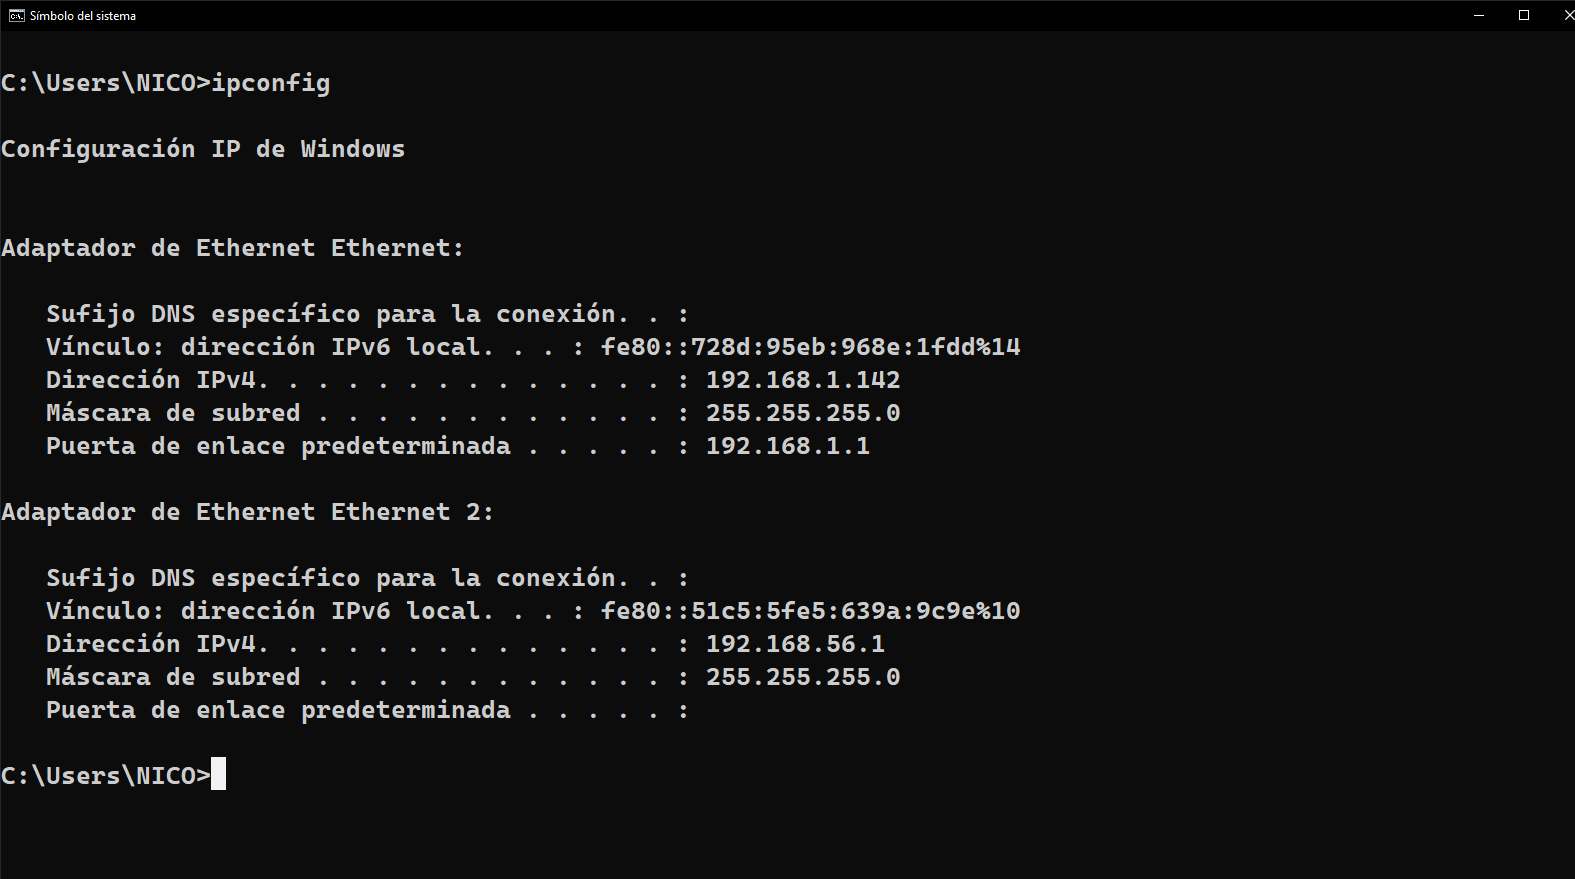
\includegraphics[width=\linewidth]{IP-Privada-preUDC.png}
        \caption{Dirección IP Privada}
    \end{subfigure}%
    \begin{subfigure}{.5\textwidth}
        \centering
        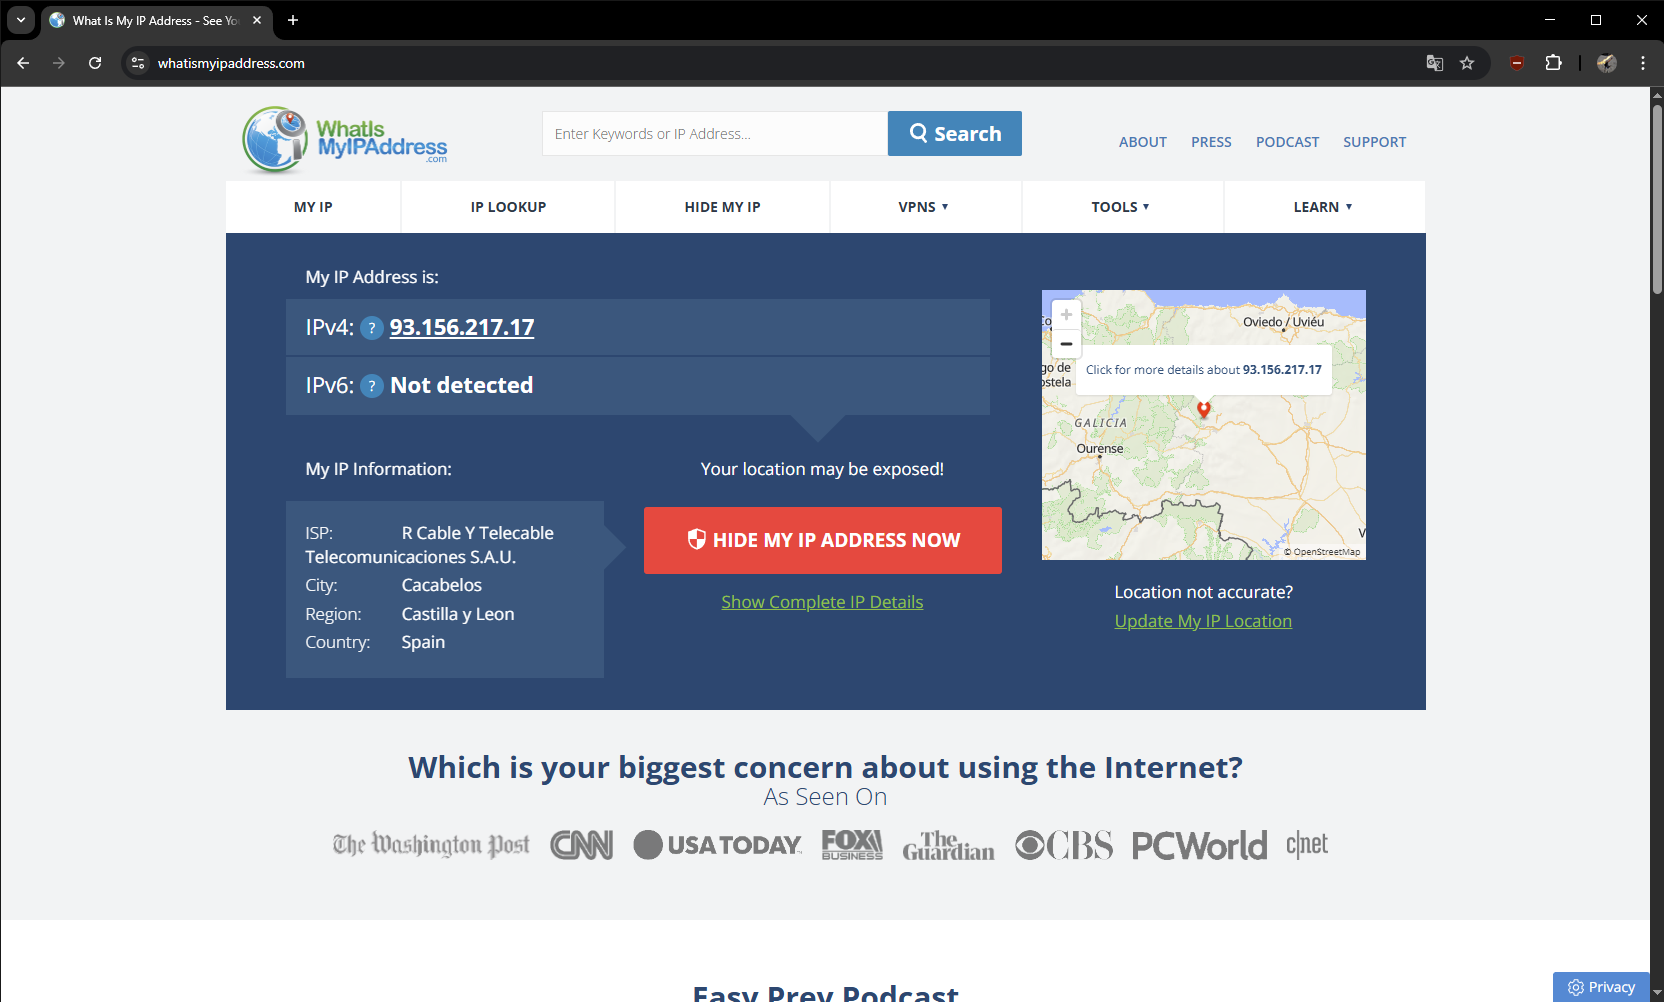
\includegraphics[width=\linewidth]{IP-Publica-preUDC.png}
        \caption{Dirección IP Pública}
    \end{subfigure}
    \caption{Direcciones IP antes de utilizar la VPN de la UDC}
    \label{fig:IPs-preUDC}
\end{figure}

\begin{figure}[H]
    \centering
    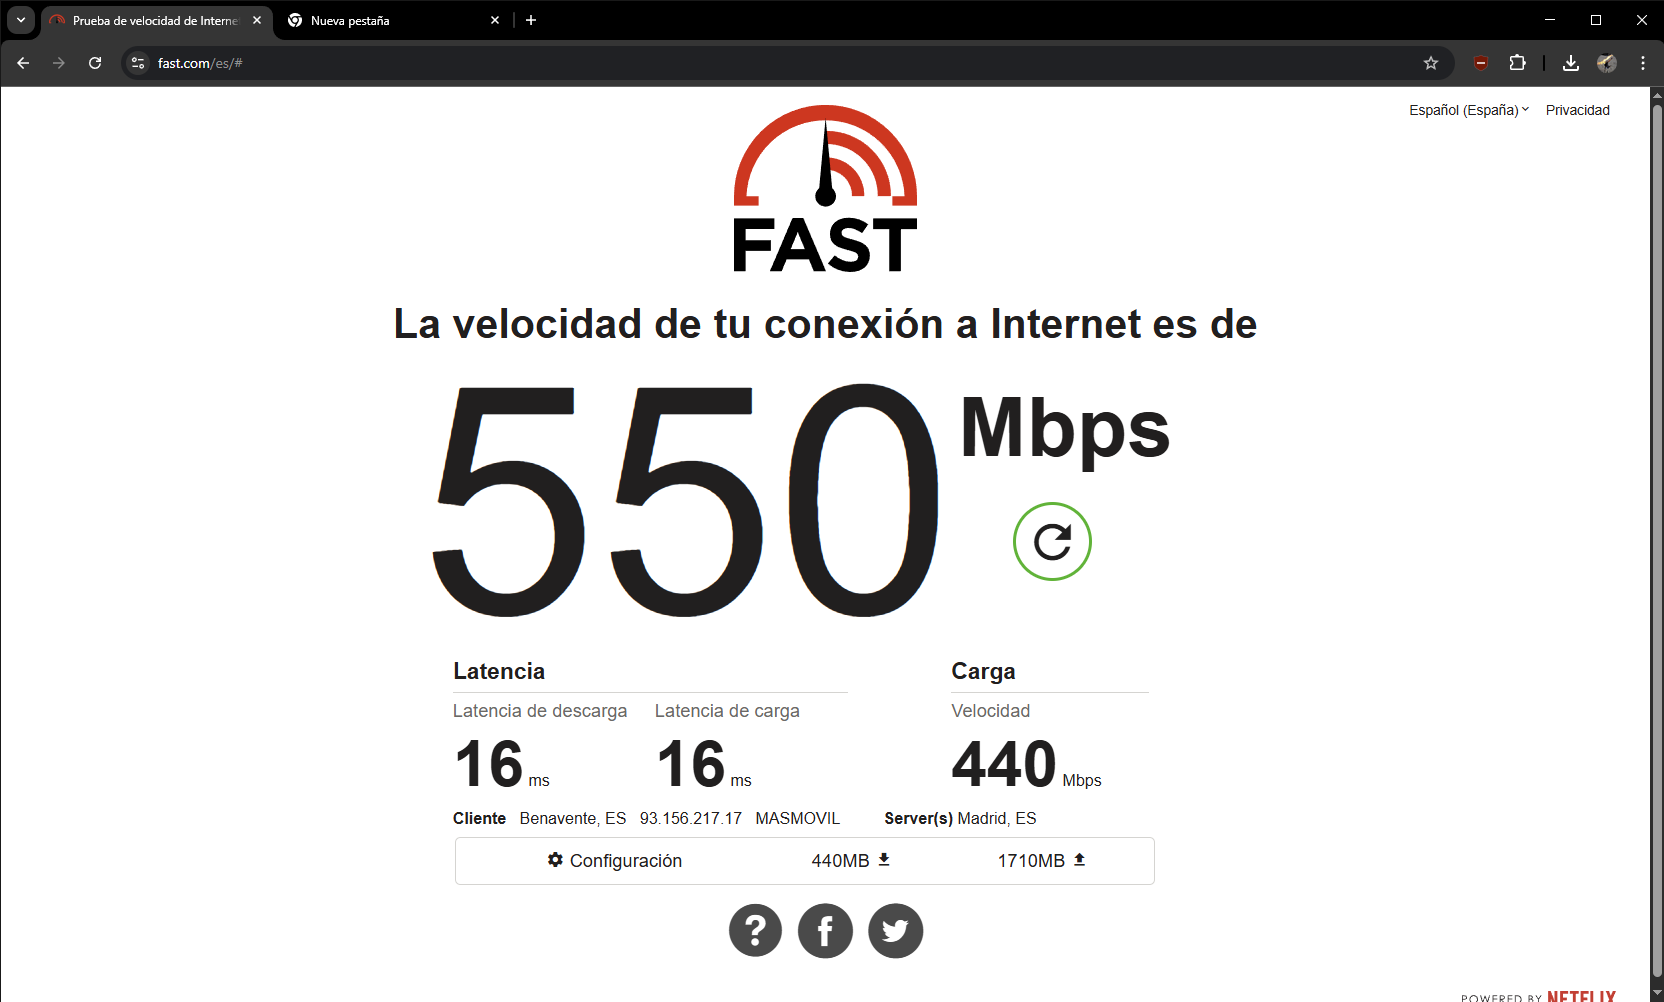
\includegraphics[width=\linewidth]{CalidadConexion-preUDC.png}
    \caption{Calidad de la conexión antes de utilizar la VPN de la UDC}
    \label{fig:Calidad-Conexión-preUDC}
\end{figure}


Observamos que las IPs privada y pública son \texttt{192.168.1.142} (primera interfaz de red) y \texttt{93.156.217.17}, respectivamente, y que contamos con una velocidad de \SI{550}{Mbps} (de descarga) y \SI{440}{Mbps} de carga, además de \SI{16}{ms} de latencia de carga/descarga.

A continuación, para poder utilizar la VPN de la UDC primero debemos instalarla y configurarla en el enlace \href{https://axudatic.udc.gal/pages/viewpage.action?pageId=45813771}{\texttt{VPN-UDC}}, dentro del apartado \texttt{`Instalación e configuración'}.

Con el cliente de VPN instalado, nos conectamos y reexaminamos los parámetros de la conexión, tal y como muestran las figuras \ref{fig:IPs-VPN-UDC} y \ref{fig:Calidad-Conexión-VPN-UDC}.

\begin{figure}[H]
    \centering
    \begin{subfigure}{.5\textwidth}
        \centering
        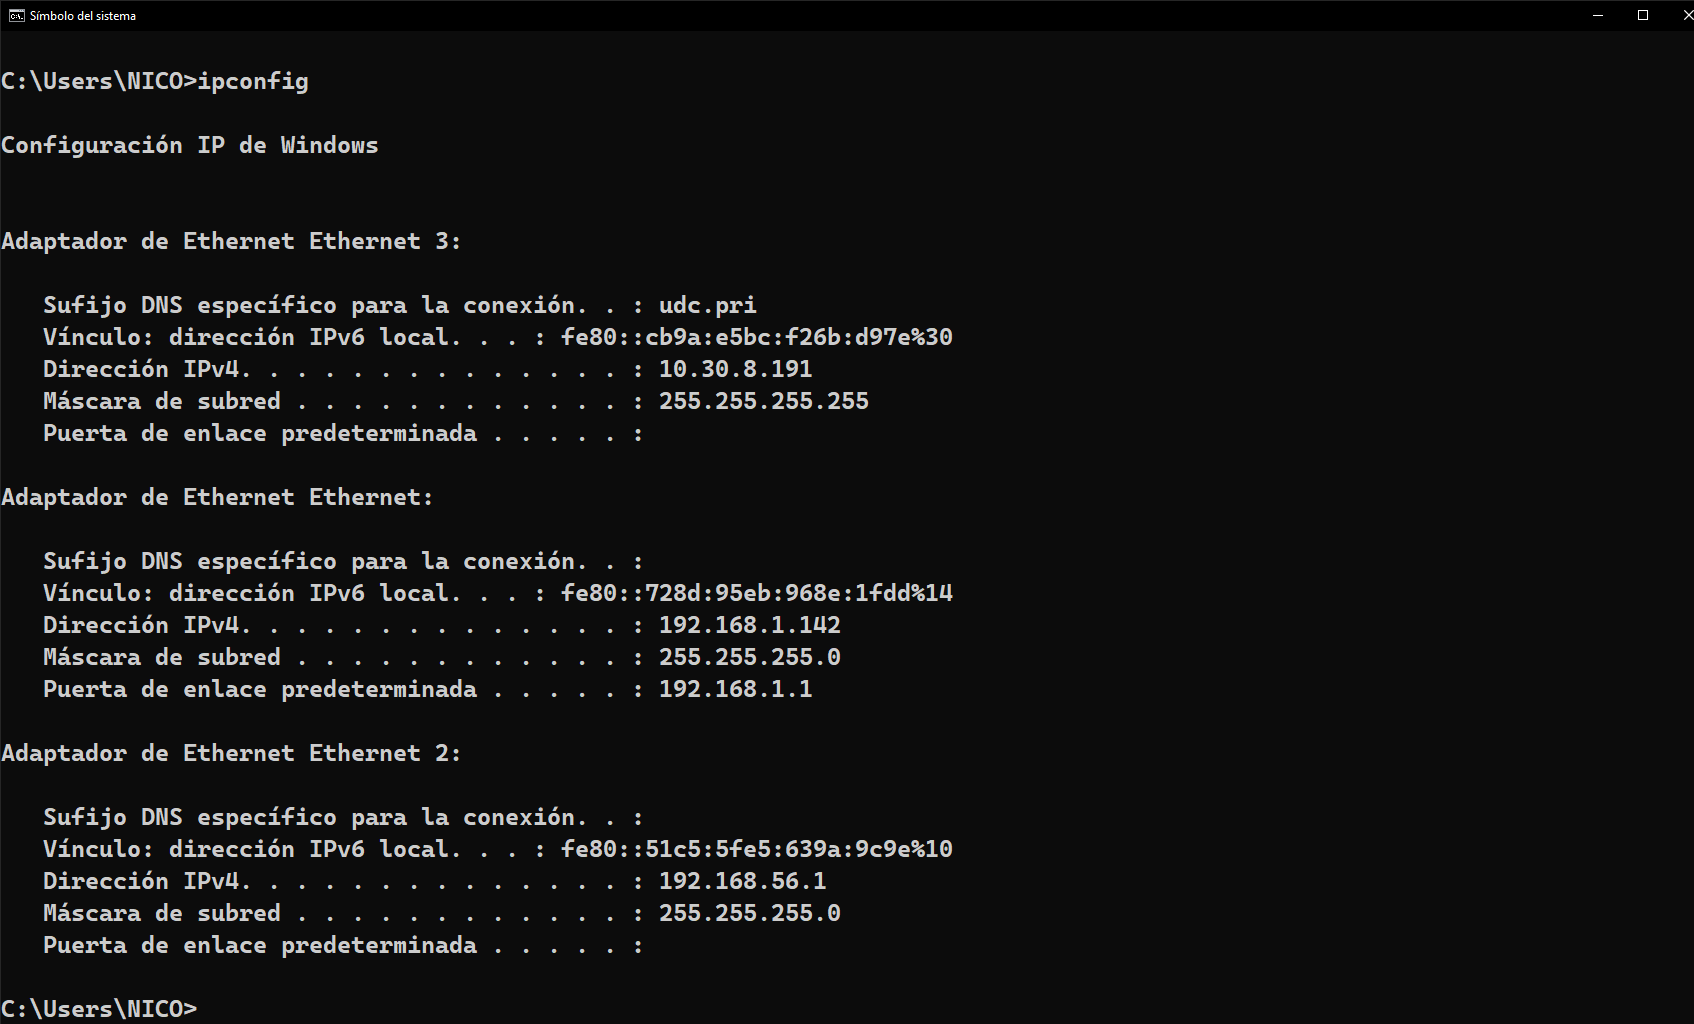
\includegraphics[width=\linewidth]{IP-Privada-VPN-UDC.png}
        \caption{Dirección IP Privada}
    \end{subfigure}%
    \begin{subfigure}{.5\textwidth}
        \centering
        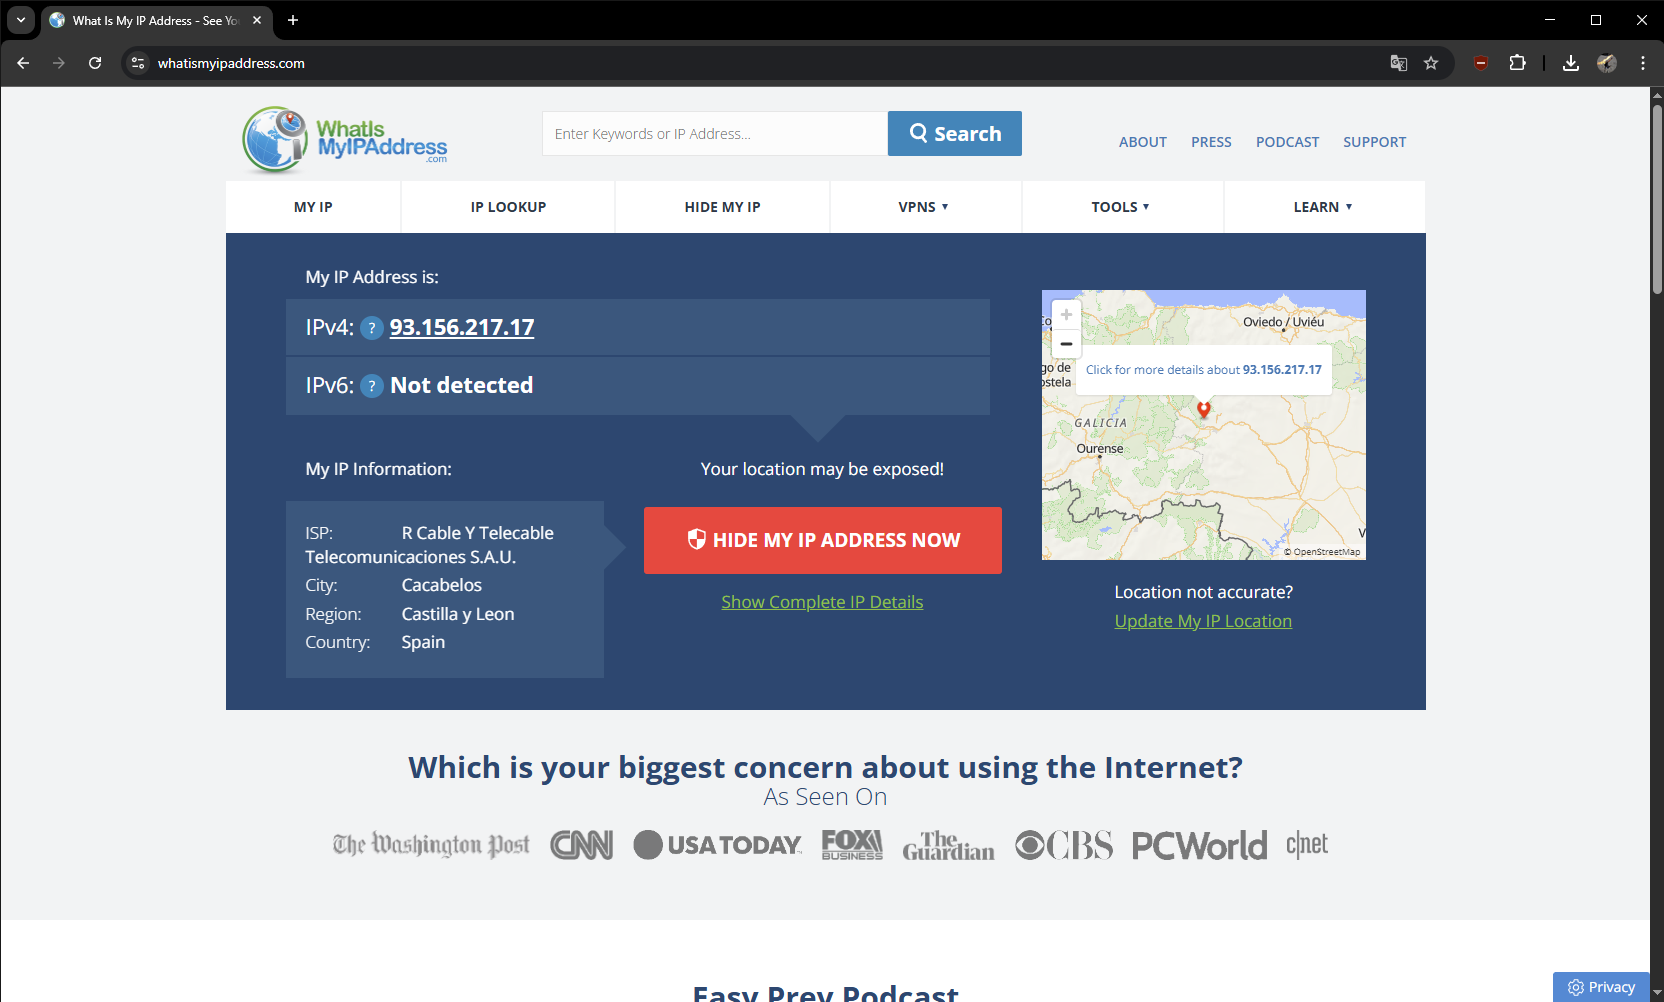
\includegraphics[width=\linewidth]{IP-Publica-VPN-UDC.png}
        \caption{Dirección IP Pública}
    \end{subfigure}
    \caption{Direcciones IP antes de utilizar la VPN de la UDC}
    \label{fig:IPs-VPN-UDC}
\end{figure}

\begin{figure}[H]
    \centering
    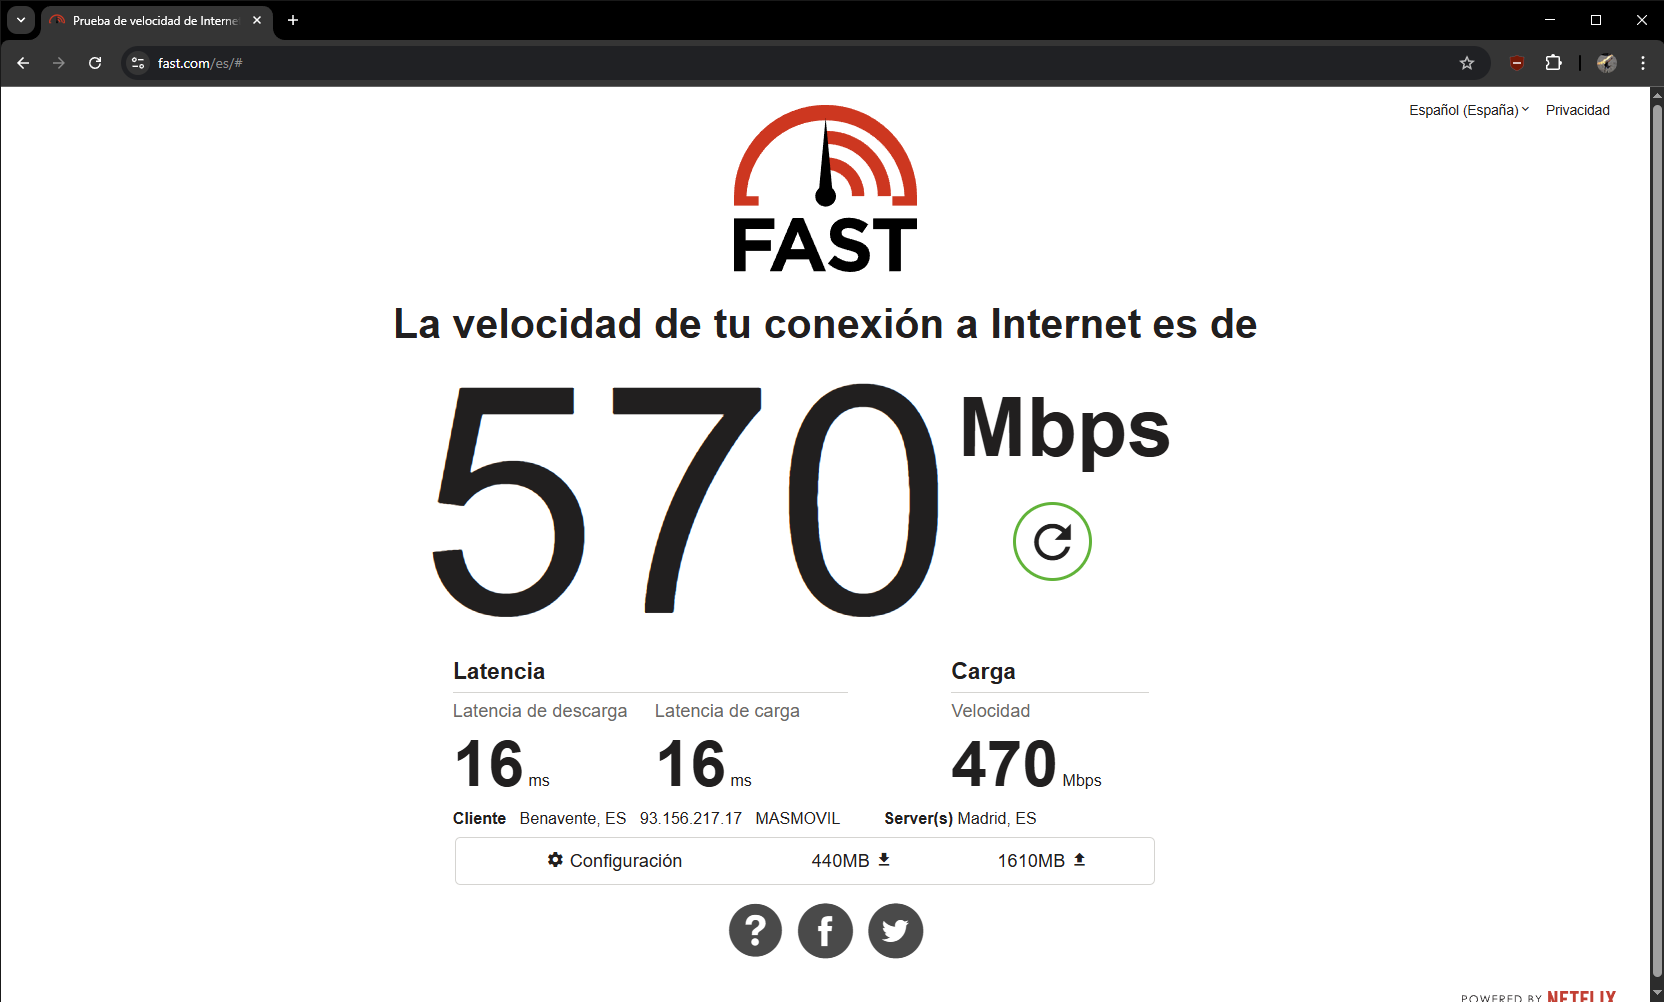
\includegraphics[width=\linewidth]{CalidadConexion-VPN-UDC.png}
    \caption{Calidad de la conexión antes de utilizar la VPN de la UDC}
    \label{fig:Calidad-Conexión-VPN-UDC}
\end{figure}


Como podemos ver, la calidad de la red no cambia demasiado, de hecho en el caso de las capturas mejoran las velocidades de carag y descarga, aunque estos resultados varían al realizarlos varias veces.
Esto concuerda con lo esperado, ya que nos encontramos cerca de la UDC.

Lo que sí llega a cambiar son las interfaces de red. Vemos que se genera una nueva interfaz de red (que lleva el sufijo DNS \texttt{udc.pri}), que corresponde a la actividad de la VPN. Su IP (privada) es \texttt{10.30.8.191/32}.
En cambio, la IP pública no cambia al pasar a utilizar la VPN.
